\documentclass[11pt, letterpaper]{report}
\usepackage[hmargin=1in, vmargin=1in]{geometry}
\usepackage[pdftex]{graphicx}
\usepackage{pdfpages}
\usepackage{listings}
\usepackage{fixltx2e}
\usepackage{fancyhdr}
\usepackage{amsmath}
\usepackage{hyperref}
\hypersetup{colorlinks=false}
\hypersetup{pdfborder = {0 0 0}}
\pagestyle{fancy}
\fancyhf{}
\lhead{Team Dijkstra}
\chead{t10 - Defect Database Design}
\rhead{Page \thepage}

\begin{document}

\title{\begin{center}
\line(1,0){450}
\end{center} \hfill \\ \Huge{Team Dijkstra }\\ \small{Crist - Ghodratnama - Howell - Sung} \\ \hfill \\ \hfill \\ \hfill \\ \huge{t10 - Defect Database Design} \\ \hfill \\ \hfill  \\ \Large{Software Engineering II} \\ \small{Spring 2013} \\ \begin{center}
\line(1,0){450}
\end{center}\small{\textit{``Elegance is not a dispensable luxury but a quality that decides between success and failure.'' \\- Edsger Dijkstra}}}
\date{ }

\maketitle
\newpage

\begin{description}

\item[\Large{Overview}] \hfill \\ \hfill \\
The document is designed to outline the procedure required for appropriately logging defects into the logging system provided and to ensure accurate, and correct information is obtained by the individuals working to resolve the conflict as well as those who reference the information in the future.  Standardizing this information will allow for points of reference in order to obtain the needed information in a timely and concise manner.  Detailed information is paramount to the accuracy of resolving such issues and reduce the time that is spent correcting the issue as well as allow for reference if the issue occurs again within the development process. \hfill \\ \hfill \\
\item[\Large{The Systems}] \hfill \\ \hfill \\
Logging of information will occur on 3 separate systems, of which will intuitively allow for quick reference based on the level of detail needed in order to resolve the issues. \hfill \\

\begin{itemize}
	\item WIKI Page - Lowest level of detail.
	\item Change Log - Moderate level of detail.
	\item Defect Log - High level of detail.
\end{itemize} \hfill \\ \hfill \\

Every defect has 6 items of information relating to it: reproduction, test to catch, discoverer, date, priority, and repair history.  Each of the three systems use this information, but not all of it.  The following sections will describe what data is contained and used accordingly along with a description of its purpose.

\textbf{WIKI Page} \hfill \\ \hfill \\
WIKI pages are generated for every module.  The information contained on these pages are in relation to the actions that are taken upon the module, the structure and other critical reference information that is required.  The change log is also reflected on this page, but not to the extent in which the change log in the file details.  Since there is no code that is made available on this page, other than points of access, the change log is merely a mention of changes that have occured within the file to correct code.  As a result this information is not of a high level of detail and is considered the lowest level of detail for information regarding the bugs and corrections made.  It can be used as a quick search area to find items in relation to a module that may have occured in the past to locate potential problems are revisit problem that may have deemed to be corrected. \hfill \\ \hfill \\
\underline{WIKI Change Log Format:} \hfill \\
\texttt{Name: \$discoverer, Date: YYYY-MM-DD, Comment: \$RepairHistory} \hfill \\ \hfill \\
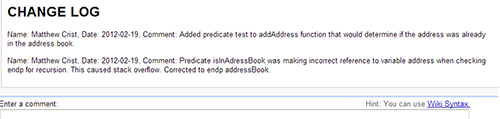
\includegraphics{change_log---wiki}
\begin{itemize}
	\item \$discoverer - The individual who took corrective action in the module.
	\item \$RepairHistory - The corrective action that was taken within the module.
\end{itemize}
** These items are recorded under the subsection "CHANGE LOG" on the wiki page to their respective modules. \hfill \\ \hfill \\
\textbf{Change Log} \hfill \\ \hfill \\
The change log is contained within the source code file in which the changes were made.  These changes should reflect the problem that occured as well as the corrective action that was taken.  The date is also included in the change as a timeline illustration of changes that have occurred during the file's conception.  While not listing the person who changed the code, it does bring to context the source code that was changed, which can be quickly identified by the developer who is referencing the change log.  All change log information is contained within the global commenting section in the source file. \hfill \\ \hfill \\
\underline{Source Change Log Example:} \hfill \\ \hfill \\
\texttt{;;;;;;;;;;;;;;;;;;;;;;;;;;;;;;;;;;;;;;;;;;;;;;;;;;;;;;;;;;;;;;;;;;;;;;;;;;;} \hfill \\
\texttt{; register-user.lisp                                                       } \hfill \\
\texttt{;                                                                          } \hfill \\
\texttt{; Created on February 14, 2013 by Matthew A. Crist.                        } \hfill \\
\texttt{;                                                                          } \hfill \\
\texttt{; Purpose:                                                                 } \hfill \\
\texttt{; This file contains the function that are essential to acquiring address  } \hfill \\
\texttt{; book information and storing entries into the address book.              } \hfill \\
\texttt{;                                                                          } \hfill \\
\texttt{; CHANGE LOG:                                                              } \hfill \\
\texttt{; -------------------------------------------------------------------------} \hfill \\
\texttt{; 2013-02-19 - Predicate isInAddressBook was making incorrect reference to } \hfill \\
\texttt{;              variable address when checking endp for recursion.  This    } \hfill \\
\texttt{;              caused stack overflow.  Correct reference to addressBook    } \hfill \\
\texttt{;              which is of type list.                                      } \hfill \\
\texttt{;                                                                          } \hfill \\
\texttt{; 2013-02-19 - Added predicate test to addAddress function in order to     } \hfill \\
\texttt{;              prevent a redundant addition to the address-book.           } \hfill \\
\texttt{;                                                                          } \hfill \\
\texttt{;;;;;;;;;;;;;;;;;;;;;;;;;;;;;;;;;;;;;;;;;;;;;;;;;;;;;;;;;;;;;;;;;;;;;;;;;;;} \hfill \\
\hfill \\
\underline{Change Log Format:} \hfill \\ \hfill \\
\texttt{YYYY-MM-DD - \$RepairHistory}
\begin{itemize}
	\item \$RepairHistory - the corrective action and short explaination of issue.
\end{itemize} \hfill \\ \hfill \\
\textbf{Defect Log} \hfill \\ \hfill \\
The defect log is not only a point of reference but also a tool that can be used to collaborate on corrective action in order to squash any bugs that occur in the software.  It can also be used to inform others of potential issues with the subsystems in which they are developing in relation to other subsystems or identifiable problems that have occured from other subsystems using that module.  The defect log not only contains the initial issue located, but also all corrective action taken, timestamps for correction and escalation of priority as well as the individuals involved in the corrective action.  Though the source is not exposed, detailed information is explained during the reported and resolution process.\hfill \\ \hfill \\
There are a number of fields that are available for reporting issues.  All issues are tracked via the "Issues" tab located on the Google source project page (https://code.google.com/p/spring-2013-se2-dijkstra/issues/list).  Each defect contains the following information:\hfill \\ \hfill \\
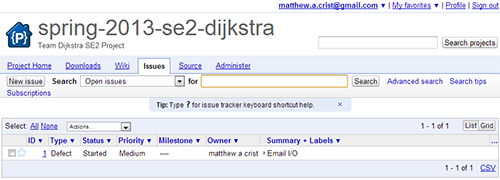
\includegraphics[width=500px,height=180px]{defect_list---defect-log}
\begin{itemize}
	\item \$ID - id that is assigned automatically by the defect database for uniqueness.
	\item \$Type - the type of issue that is assigned to the defect by the submitter.
	\item \$Status - the status towards resolution of this defect.
	\item \$Priority - the prioritization level for this defect.
	\item \$Milestone - milestones assigned to the completion of this defect for completion.
	\item \$Owner - the submitter of the defect.
	\item \$Summary - general information about the defect.
\end{itemize}
\hfill \\ \hfill \\
The information that is contained on the listings page will be filed upon the creation of the defect.  Creating a defect can be done by clicking the "New Issue" button located in the upper left section of the defect listing.  From there, the files that are made available will allow you to fill in the information as listed above.\hfill \\ \hfill \\
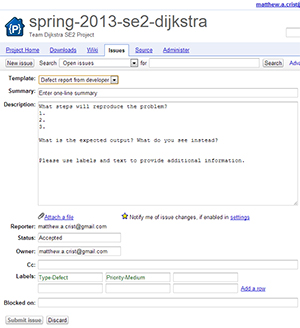
\includegraphics{defect_entry---defect-log} \hfill \\ \hfill \\
When the issue is created, it is important that the developers associated with the project check the defect log for new updates in order to ensure they are resolved or will be resolved.  You can CC the development team of issue by typing in their email addresses so they will be notified on creation of the defect.
\end{description}
\end{document}